\chapter{NLP Foundations: Getting Text and Measuring It}
\label{ch:nlp-foundations}

\chapterguide%
  {Manipulate Python strings, and know what a controlled experiment is.}
  {describe an NLP pipeline from raw input to task output; explain why text normalisation comes before any comparison; compute Levenshtein distance by hand and turn it into character error rate; design a fair before/after comparison of a preprocessing step; and separate segmentation failures from recognition failures in an OCR error analysis.}

Natural language processing (NLP) starts before there is any language to process, because text has to come from somewhere: keystrokes, speech or images. Lab~6 applies optical character recognition to 89 photographs of handwritten medicine names and asks: \emph{how good is the resulting text, and how should we measure it?}

\section{Every NLP task is a pipeline}

NLP systems acquire text, normalise it, build a representation, apply a task model and evaluate the output (\figref{fig:nlp-pipeline}).

\begin{analogy}
Think of an assembly line. A part that falls off at the first station is simply missing at every station after it, however good those later stations are. Early errors in NLP work the same way: no downstream model can use a word that OCR never saw.
\end{analogy}

\begin{utpfig}[The NLP pipeline]{Lab~6 covers acquisition, normalisation and OCR measurement. Lab~7 starts with clean text and builds a representation and classifier.}{fig:nlp-pipeline}
\begin{tikzpicture}[scale=0.99,transform shape,
  b/.style={draw=UTPBlue,fill=UTPPaleBlue,rounded corners=2mm,minimum width=2.20cm,minimum height=1.0cm,align=center,font=\small\color{UTPNavy}},
  arr/.style={-{Stealth[length=2mm]},thick,draw=UTPTeal}
]
\node[b] (acq) {Acquire\\\scriptsize photo, audio, keyboard};
\node[b,right=0.26cm of acq] (norm) {Normalise\\\scriptsize case, punctuation, tokens};
\node[b,right=0.26cm of norm] (rep) {Represent\\\scriptsize counts, n-grams, vectors};
\node[b,right=0.26cm of rep] (model) {Model\\\scriptsize classify, translate, search};
\node[b,right=0.26cm of model] (eval) {Evaluate\\\scriptsize against references};
\draw[arr] (acq)--(norm); \draw[arr] (norm)--(rep); \draw[arr] (rep)--(model); \draw[arr] (model)--(eval);
\draw[utpbrace,decoration={mirror},draw=UTPOrange] (-1.3,-0.75) -- (3.9,-0.75);
\node[font=\scriptsize\color{UTPOrange},anchor=north] at (1.3,-0.95) {Lab~6: OCR, normalisation, measurement};
\draw[utpbrace,decoration={mirror},draw=UTPGreen] (4.1,-0.75) -- (12.0,-0.75);
\node[font=\scriptsize\color{UTPGreen},anchor=north] at (8.1,-0.95) {Lab~7: bag of words, Naive Bayes, evaluation};
\end{tikzpicture}
\end{utpfig}

\section{Optical character recognition as text acquisition}

\term{OCR} converts images to strings. Tesseract, the engine used in the lab, works in two stages. \term{Segmentation} locates the text on the page, and a neural \term{recognition} stage reads what it found. Keeping the stages apart in your head matters, because they fail differently: one misses text altogether, the other misreads it.

Lab~6 fixes \texttt{--oem 1} (neural recognition) and \texttt{--psm 7} (treat the image as a single line of text) for every cropped name. Holding these settings constant isolates the effect of preprocessing.

\begin{intuition}
Tesseract was built mainly for print, not for cursive on lined paper. Asking it to read a doctor's handwriting is like asking someone who learned a language from textbooks to follow a fast regional accent. Downstream processing cannot reliably recover what the recogniser missed.
\end{intuition}

\section{Normalisation before comparison}

``Tab Azimax'' and ``tab azimax'', or ``40 mg'' and ``40mg'', differ as strings. If we compared raw strings, a capital letter would count as an error just like a wrong drug name. Lab~6 therefore reduces predictions and references to lowercase letters and digits before comparing them:

\lstinputlisting[style=utppython,firstline=69,lastline=70]{all_experiments/lab06_handwriting_ocr_worked.py}

This rule excludes case, spacing and punctuation from the error count. A task that must distinguish ``40 mg'' from ``4 0mg'' needs a different rule, and its scores are not directly comparable with these. The choice is visible in the numbers: on the raw baseline the character error rate is 0.88 with this normaliser, 0.88 if spaces are kept, and 0.93 with no normalisation at all.

\begin{keyidea}
Normalise both sides identically, decide in advance which differences count as errors, and write the rule down. A metric is only meaningful relative to the normalisation it was computed under.
\end{keyidea}

\section{Measuring text quality: edit distance}

\term{Exact match} requires identical normalised strings, and none of the 89 baseline predictions qualifies. That single number hides a lot. Reading \texttt{dicloran} as \texttt{diclorew} is nearly right, while reading it as nothing at all is useless, yet exact match scores both as zero. We need a graded measure.

\term{Levenshtein distance} gives one: the minimum number of single-character insertions, deletions and substitutions needed to turn one string into the other. Imagine a proofreader correcting the OCR output with a red pen and charging one unit per mark. The distance is the smallest possible bill (\figref{fig:levenshtein}).

\begin{utpfig}[Levenshtein distance by dynamic programming]{The table for turning the reference \texttt{nims} into the OCR output \texttt{nidu}, as Lab~6's baseline actually read it. Cell $(i,j)$ holds the cost of matching the first $i$ characters of the reference with the first $j$ of the prediction: one more than the cell above (delete), one more than the cell to the left (insert), or the diagonal plus one if the characters differ (substitute). The answer, 2, is in the bottom-right corner: substitute \texttt{m}$\to$\texttt{d} and \texttt{s}$\to$\texttt{u}.}{fig:levenshtein}
\begin{tikzpicture}[font=\small]
\def\W{0.78}
\foreach \c [count=\ci from 1] in {n,i,d,u}{\node[font=\bfseries\color{UTPOrange}] at (\W*\ci,\W*0.85) {\c};}
\foreach \r [count=\ri from 1] in {n,i,m,s}{\node[font=\bfseries\color{UTPBlue}] at (-\W*0.85,-\W*\ri) {\r};}
\foreach \row [count=\ri from 0] in {{0,1,2,3,4},{1,0,1,2,3},{2,1,0,1,2},{3,2,1,1,2},{4,3,2,2,2}}{
  \foreach \v [count=\ci from 0] in \row{
    \ifnum\ri=\ci
      \node[utphot,minimum width=\W cm,minimum height=\W cm,font=\scriptsize\bfseries] at (\W*\ci,-\W*\ri) {\v};
    \else
      \node[utpcell,minimum width=\W cm,minimum height=\W cm,font=\scriptsize] at (\W*\ci,-\W*\ri) {\v};
    \fi
  }
}
\node[utplabel,anchor=north,color=UTPBlue] at (-\W*0.85,-\W*4.6) {reference};
\node[utplabel,anchor=south,color=UTPOrange] at (\W*2.5,\W*1.3) {prediction};
\node[utplabel,anchor=west,align=left,text width=6.2cm] at (\W*5.4,-\W*1.2)
  {$D[i,j]=\min\big(D[i-1,j]+1,\ D[i,j-1]+1,\ D[i-1,j-1]+[r_i\neq p_j]\big)$\\[4pt]
   The highlighted diagonal is the cheapest path: match \texttt{n}, match \texttt{i}, substitute, substitute.\\[4pt]
   Distance $=2$; normalised by the longer length, $2/4=0.5$.};
\end{tikzpicture}
\end{utpfig}

The lab's implementation computes that table one row at a time, keeping only the previous row:

\lstinputlisting[style=utppython,firstline=104,lastline=112]{all_experiments/lab06_handwriting_ocr_worked.py}

The lab reports three distance-based metrics and a separate blank count:

\begin{utptable}
\begin{tabularx}{\linewidth}{@{}>{\bfseries\leavevmode\color{UTPNavy}}m{0.30\linewidth}m{0.30\linewidth}X@{}}
\toprule
\rowcolor{UTPPaleBlue!92}
\utpth{Metric} & \utpth{Definition} & \utpth{Answers} \\
\midrule
Exact-match accuracy & Fraction of images with distance $0$ & How often is the name usable as-is? \\
Mean normalised edit distance & Mean over images of distance $/$ longer length; in $[0,1]$ & How wrong is a typical image? \\
Character error rate (CER) & Total edits $/$ total reference characters; can exceed $1$ & How many corrections per 100 reference characters? \\
Blank predictions & Images whose normalised prediction is empty & How often did segmentation find nothing? \\
\bottomrule
\end{tabularx}
\end{utptable}

\begin{workedexample}
Take two images. Reference \texttt{nims} is read as \texttt{nidu}: 2 edits on 4 characters. Reference \texttt{tabnims100mg} is read as nothing: 12 edits on 12 characters.

\[
\text{mean normalised distance}=\frac{2/4+12/12}{2}=0.75,
\qquad
\text{CER}=\frac{2+12}{4+12}=0.875.
\]

The mean treats both images equally. CER pools the characters, so the long name counts for more.
\end{workedexample}

\begin{pitfall}
CER is a ratio of totals, so long references dominate it. The normalised distance is a mean of per-image ratios, so every image counts equally. The two can move in opposite directions on the same data. Report both, and say which one a decision rests on.
\end{pitfall}

\section{A controlled preprocessing experiment}

The baseline has CER near $0.9$ and 44 blank predictions. Lab~6 tests one fixed preprocessing pipeline: grayscale, a 20-pixel white border, a width cap and $1.5\times$ enlargement. These steps target colour noise, text touching the image edge and character size, and they leave the OCR settings alone.

Use the same 89 images, the same normalisation and the same OCR configuration, so that only the image preprocessing changes. A fair experiment changes one thing.

\begin{utptable}
\begin{tabularx}{\linewidth}{@{}>{\bfseries\leavevmode\color{UTPNavy}}m{0.30\linewidth}>{\centering\arraybackslash}X>{\centering\arraybackslash}X>{\centering\arraybackslash}X>{\centering\arraybackslash}X@{}}
\toprule
\rowcolor{UTPPaleBlue!92}
\utpth{Pipeline} & \utpth{Exact match} & \utpth{Norm.\ edit distance} & \utpth{CER} & \utpth{Blank} \\
\midrule
Raw images & 0.000 & 0.860 & 0.881 & 44 \\
Grayscale, border, resize & 0.011 & 0.767 & 0.788 & 15 \\
\bottomrule
\end{tabularx}
\end{utptable}

Blanks fall from 44 to 15 and CER falls by about $0.09$, but only one image, \texttt{ostium}, becomes an exact match. Look past the totals and the picture is more mixed. Measured by edits, 43 images improved, 18 got worse and 28 did not change. Thirty-four images that were blank now yield text, while 5 that yielded text are now blank: \texttt{tab mesulid}, for instance, was read as \texttt{wos Mesulia} on the raw image and not at all after preprocessing. On balance preprocessing helps segmentation find text, and it leaves substantial recognition errors behind.

\section{Error analysis: which stage failed?}

Lab~6 sorts predictions by normalised edit distance and tags the worst cases. It keeps all 89 samples, records any OCR-engine exception instead of dropping the image, and assigns each difficult case one of three reproducible labels. If Tesseract is not installed, the notebook identifies the run as \emph{cached} and loads the validated predictions supplied with the course package; it never presents cached text as a live run.

\begin{description}
  \item[Engine error.] Tesseract rejects an individual image. The sample stays in the benchmark as a failed recognition, with the error recorded in \texttt{predictions.csv}.
  \item[No text detected.] An empty normalised prediction suggests missed text, for example from faint strokes, low contrast or slanted writing. Preprocessing may help. Seven of the eight worst preprocessed cases are of this kind.
  \item[Character confusion.] Text is returned but misread: \texttt{provas} as \texttt{Pras}, or \texttt{starcox 90} as \texttt{Stak Oe 90}. Persistent handwriting errors point to the need for a recogniser trained on handwriting.
\end{description}

Save the six hardest images with their references and predictions, so readers can check the tags for themselves.

\begin{keyidea}
Attribute each failure to the stage that produced it. The fix for ``no text found'' is different from the fix for ``wrong text found'', and an aggregate score cannot tell them apart.
\end{keyidea}

\section{Fitness for purpose}

The benchmark shows a poor fit between printed-text OCR and cursive handwriting, not evidence for clinical use. Misread medicine names or doses can cause real harm. Clinical transcription would require a handwriting-specific recogniser, representative data, held-out validation, privacy controls and human review of uncertain readings.

\begin{chapterrecap}
\begin{itemize}
  \item NLP is a pipeline, and errors made early cannot be repaired later.
  \item Normalise references and predictions by one written rule before comparing them. A metric means nothing without it.
  \item Levenshtein distance counts the fewest single-character edits, and normalised distance and CER aggregate it in two different ways.
  \item Change one thing at a time. Preprocessing cut blanks from 44 to 15 but barely moved exact matches.
  \item Attribute each failure to segmentation or recognition, because they need different fixes.
\end{itemize}
\end{chapterrecap}

\begin{quickcheck}
\begin{enumerate}
  \item How do an engine error, a blank prediction, and \texttt{nims} being read as \texttt{nidu} differ?
  \item Compute the Levenshtein distance between \texttt{breeky} and \texttt{beeky}, and the normalised distance.
  \item Why must the OCR configuration stay fixed when the preprocessing pipeline is tested?
  \item After preprocessing, CER fell by $0.09$ but exact-match accuracy rose by only one image. What does that pattern say about which stage improved?
  \item The lab's normaliser deletes spaces. Name a task for which that would be the wrong choice.
\end{enumerate}
\end{quickcheck}

\begin{checkanswers}
\begin{enumerate}
  \item An engine error is a recorded runtime failure of Tesseract on that image; a blank prediction means the segmenter found no text line; \texttt{nidu} means a line was found but the recogniser misread its characters. Only the last is a recognition failure.
  \item Delete one \texttt{r}: distance $1$. Normalised by the longer length, $1/6\approx0.17$.
  \item Otherwise an improvement could come from the engine settings rather than from the images. A controlled experiment changes one factor at a time.
  \item The segmentation stage improved, since many more images now yield some text, while the recognition stage still misreads cursive, so few of those texts are exactly right.
  \item Any task in which spacing carries meaning: distinguishing ``40 mg'' from ``4 0mg'', counting words, or matching multi-word names.
\end{enumerate}
\end{checkanswers}

\labsection{6}{NLP Foundations: Handwriting OCR Evaluation}{sec:lab06-nlp-a}

\begin{labproject}{Evaluate OCR on real handwritten medicine names}
\textbf{Read first.} Chapter~\ref{ch:nlp-foundations}.\\
\textbf{Goal.} Benchmark OCR on 89 labelled images, test one controlled preprocessing pipeline, and classify the failures.\\
\textbf{Scenario.} A clinic wants to digitise handwritten medicine names before storage or search.\\
\textbf{Data.} \texttt{all\_datasets/lab06-ocr-handwritten-prescription.zip}: one label CSV and 89 images. The notebook extracts it next to the archive.\\
\textbf{Notebook.} \texttt{all\_experiments/lab06\_handwriting\_ocr\_worked.ipynb}.\\
\textbf{Hand in.} The executed notebook, the \texttt{results/lab06/} folder and a short conclusion, as listed in the checklist at the end of this sheet.
\end{labproject}

\begin{labmode}
\begin{enumerate}
  \item Activate your course environment and confirm that the zip is in \texttt{all\_datasets/}. Do not extract it yourself; the notebook does that.
  \item \textbf{Install the Tesseract OCR engine.} This is the one lab that needs software beyond Python. The \texttt{pytesseract} package in \texttt{requirements.txt} is only a wrapper around it. Use the line for your system, then reopen the terminal and check the version.
  \item Start Jupyter from \texttt{all\_experiments/}, open the notebook, and choose \textbf{Restart Kernel and Run All Cells}.
\end{enumerate}
\begin{lstlisting}[style=utpterminal]
# Windows (PowerShell)
winget install --id UB-Mannheim.TesseractOCR -e

# macOS
brew install tesseract

# Debian or Ubuntu
sudo apt install tesseract-ocr

# Every system: check it, then start the lab
tesseract --version
cd all_experiments
jupyter lab
\end{lstlisting}
On Windows the notebook also looks in \texttt{C:\textbackslash Program Files\textbackslash Tesseract-OCR}, so it finds a default install even if the terminal does not.
\end{labmode}

\begin{pitfall}
\textbf{Live or cached?} With Tesseract and its Python wrapper installed, this lab performs live recognition, and the first printed line says \texttt{OCR mode: live}. Otherwise it analyses the supplied predictions in \texttt{results/lab06/predictions.csv} and says \texttt{OCR mode: cached}. A cached run can reproduce the saved comparison and every metric, but it cannot test a new preprocessing choice. Never describe a cached run as new OCR inference. Keep \texttt{predictions.csv} in place, because cached mode reads it.
\end{pitfall}

\courselabflow{Extract images}{Run OCR}{Normalise text}{Compare errors}


\labroutine

\begin{yourturn}
\textbf{Warm-up on paper.} The raw baseline reads \texttt{dicloran} as \texttt{diclerew}. Work out the Levenshtein distance by hand, using the table method of \figref{fig:levenshtein}, and then the normalised distance.

\emph{Answer.} Substitute \texttt{o}$\to$\texttt{e}, \texttt{a}$\to$\texttt{e} and \texttt{n}$\to$\texttt{w}: distance 3. Both strings have 8 characters, so the normalised distance is $3/8=0.375$.
\end{yourturn}

\textbf{Setup.} Run the imports and path setup first, and keep this kernel state for the later questions. In the script version the first seven lines also set the working directory.
\lstinputlisting[style=utppython,firstline=1,lastline=7]{all_experiments/lab06_handwriting_ocr_worked.py}
\lstinputlisting[style=utppython,firstline=8,lastline=40]{all_experiments/lab06_handwriting_ocr_worked.py}
\begin{refoutput}
\begin{lstlisting}[style=utpterminal]
OCR mode: live | Tesseract 5.5.3.20260724 at C:\Program Files\Tesseract-OCR\tesseract.exe
\end{lstlisting}
\end{refoutput}

\begin{labquestion}{1}{Validate the archive}
Extract the archive next to itself, load the label file, check that all 89 labelled images exist exactly once, report the number of unique labels, and show a 3-by-3 sample grid.
\end{labquestion}
\begin{labanswer}
\courselabtrace{Compare the same images twice}{Baseline}{Original image to recognised text}{Treatment}{Preprocess image, then use the same OCR engine}{Check}{Pair both predictions with the same true label}

\lstinputlisting[style=utppython,firstline=42,lastline=64]{all_experiments/lab06_handwriting_ocr_worked.py}
\begin{labvisual}{Reference plot from the supplied notebook}
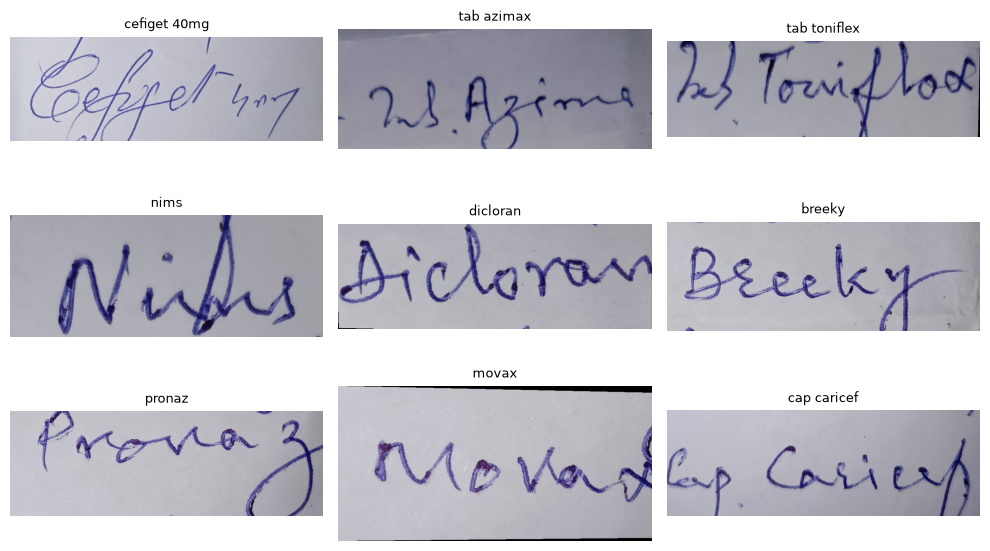
\includegraphics[width=.88\linewidth,height=5cm,keepaspectratio]{labs/visuals/06-notebook-reference.png}
\end{labvisual}
\begin{refoutput}
\begin{lstlisting}[style=utpterminal]
Labelled images: 89 | unique labels: 61
\end{lstlisting}
\end{refoutput}

\textbf{What it means.} One label file and 89 photographs, each present exactly once. The 89 labels hold 61 distinct medicine names, so some names appear several times in different handwriting. The grid shows what the engine faces: cursive, varied stroke width, uneven lighting and lined paper.
\end{labanswer}

\begin{labquestion}{2}{Run the baseline OCR}
Use one fixed Tesseract configuration for every raw image (LSTM engine, page-segmentation mode 7 = one text line) and normalise both prediction and label to lowercase letters and digits. Record a per-image engine failure instead of dropping the sample or stopping the benchmark.
\end{labquestion}
\begin{labanswer}
\lstinputlisting[style=utppython,firstline=66,lastline=102]{all_experiments/lab06_handwriting_ocr_worked.py}
\begin{refoutput}
\begin{lstlisting}[style=utpterminal]
          truth      prediction prediction_norm
0  cefiget 40mg
1    tab azimax              Ao              ao
2  tab toniflex  p53 Towid host    p53towidhost
3          nims            Nidu            nidu
4      dicloran        diclerew        diclerew
OCR engine errors: 0
\end{lstlisting}
\end{refoutput}

\textbf{What it means.} The first rows distinguish a blank recognition from a misread name while retaining every labelled image. The configuration is fixed, so any later improvement must come from the image rather than from engine tuning.
\end{labanswer}

\textbf{Connect it to the chapter.} The next questions measure the second and third boxes of this pipeline, and an error made in the first cannot be repaired by them.
% Reused from chapters/06-nlp-foundations.tex
\begin{labvisual}{Recall the chapter model}
\begin{labgraphic}
\begin{tikzpicture}[scale=0.99,transform shape,
  b/.style={draw=UTPBlue,fill=UTPPaleBlue,rounded corners=2mm,minimum width=2.20cm,minimum height=1.0cm,align=center,font=\small\color{UTPNavy}},
  arr/.style={-{Stealth[length=2mm]},thick,draw=UTPTeal}
]
\node[b] (acq) {Acquire\\\scriptsize photo, audio, keyboard};
\node[b,right=0.26cm of acq] (norm) {Normalise\\\scriptsize case, punctuation, tokens};
\node[b,right=0.26cm of norm] (rep) {Represent\\\scriptsize counts, n-grams, vectors};
\node[b,right=0.26cm of rep] (model) {Model\\\scriptsize classify, translate, search};
\node[b,right=0.26cm of model] (eval) {Evaluate\\\scriptsize against references};
\draw[arr] (acq)--(norm); \draw[arr] (norm)--(rep); \draw[arr] (rep)--(model); \draw[arr] (model)--(eval);
\draw[utpbrace,decoration={mirror},draw=UTPOrange] (-1.3,-0.75) -- (3.9,-0.75);
\node[font=\scriptsize\color{UTPOrange},anchor=north] at (1.3,-0.95) {Lab~6: OCR, normalisation, measurement};
\draw[utpbrace,decoration={mirror},draw=UTPGreen] (4.1,-0.75) -- (12.0,-0.75);
\node[font=\scriptsize\color{UTPGreen},anchor=north] at (8.1,-0.95) {Lab~7: bag of words, Naive Bayes, evaluation};
\end{tikzpicture}
\end{labgraphic}\end{labvisual}


\begin{labquestion}{3}{Measure recognition quality}
Implement Levenshtein edit distance and report, for the baseline: exact-match accuracy, mean normalised edit distance (distance divided by the longer string, so it lies in 0--1), character error rate (total edits divided by total reference characters; it can exceed 1), and the number of blank predictions.
\end{labquestion}
\begin{labanswer}
Inspect the normalisation and distance functions before interpreting the metrics:
\courselabtrace{Trace the OCR scoring fields}{1. Input / state}{Keep each filename, reference and prediction together; normalise both strings consistently.}{2. Operation}{add\_distances computes exact match and edit distances for each row; summarise aggregates the scored rows.}{3. Check}{Blank predictions remain failures. Compare baseline and preprocessed on the same labelled images.}


\lstinputlisting[style=utppython,firstline=104,lastline=133]{all_experiments/lab06_handwriting_ocr_worked.py}
\begin{refoutput}
\begin{lstlisting}[style=utpterminal]
   pipeline  exact_match  mean_norm_edit_distance  character_error_rate  blank_predictions
0  baseline        0.000                   0.8598                0.8805                 44
\end{lstlisting}
\end{refoutput}

\textbf{What it means.} Generic OCR on raw handwriting is poor: none of the 89 names is read exactly, the character error rate is close to 0.9, and 44 images yield no text. Any engine error is counted as a failed recognition, not silently removed.
\end{labanswer}

\begin{labquestion}{4}{Build one preprocessing pipeline}
Convert each image to grayscale, add a 20-pixel white border, cap the width at 1,200 pixels, and enlarge by $1.5\times$ with bicubic resampling. Save the results under \texttt{results/lab06/preprocessed/}. The OCR configuration does not change.
\end{labquestion}
\begin{labanswer}
\lstinputlisting[style=utppython,firstline=135,lastline=148]{all_experiments/lab06_handwriting_ocr_worked.py}
\begin{refoutput}
\begin{lstlisting}[style=utpterminal]
Prepared images: 89 | example size: (1800, 638) mode: L
\end{lstlisting}
\end{refoutput}

\textbf{What it means.} Each step targets a known weakness of Tesseract on photographs: grayscale removes colour noise, the border stops text touching the edge (which breaks line segmentation), the width cap bounds runtime, and the enlargement brings stroke height into the range the engine was trained on. Only the image changes.
\end{labanswer}

\begin{labquestion}{5}{Compare the two pipelines fairly}
Run OCR on the preprocessed images with the identical configuration, keep exactly the same 89 samples, save one row per image and pipeline to \texttt{predictions.csv}, and save both sets of metrics to \texttt{metrics.csv}.
\end{labquestion}
\begin{labanswer}
\lstinputlisting[style=utppython,firstline=150,lastline=156]{all_experiments/lab06_handwriting_ocr_worked.py}
\begin{refoutput}
\begin{lstlisting}[style=utpterminal]
                         exact_match  mean_norm_edit_distance    CER  blank
baseline                      0.0000                   0.8598  0.8805     44
grayscale_border_resize       0.0112                   0.7673  0.7883     15
\end{lstlisting}
\end{refoutput}

\textbf{What it means.} Preprocessing cuts the blank predictions from 44 to 15 and lowers the character error rate by about 0.09, but exact-match accuracy barely moves (one correct name out of 89): the engine now \emph{sees} text on most images yet still cannot read cursive. Because both pipelines were scored on the same 89 images with the same configuration, the difference is attributable to the preprocessing alone. Exact numbers depend on the Tesseract version; the direction of the changes should not.
\end{labanswer}

\begin{labquestion}{6}{Analyse the failures}
Take the worst preprocessed predictions by normalised edit distance and tag each as an \emph{engine error}, \emph{no text detected}, or \emph{character confusion}. Save \texttt{error\_analysis.csv} and a figure of the six hardest images.
\end{labquestion}
\begin{labanswer}
\lstinputlisting[style=utppython,firstline=158,lastline=174]{all_experiments/lab06_handwriting_ocr_worked.py}
\begin{refoutput}
\begin{lstlisting}[style=utpterminal]
Saved: ['error_analysis.csv', 'metrics.csv', 'ocr_failures.png', 'predictions.csv', 'sample_grid.png']
\end{lstlisting}
\end{refoutput}

\textbf{What it means.} Of the eight worst cases, seven are \emph{no text detected} and one is \emph{character confusion}. An engine error is a recorded runtime failure, no text detected is a segmentation failure, and character confusion is a recognition failure, and each needs a different fix. This is a benchmark of how well a model fits a domain, not evidence that generic OCR suits clinical transcription.
\end{labanswer}

\begin{yourturn}
Add new cells at the end of the notebook. Tasks 1 and 2 work in live and cached mode, because they recompute from the saved predictions. Task 3 needs live OCR.
\begin{enumerate}
  \item \textbf{Look past the totals.} Using \texttt{baseline} and \texttt{preprocessed}, count the images whose edits improved, worsened or stayed the same, and how many went from blank to text and from text to blank.
  \item \textbf{Change the normaliser.} Recompute CER for both pipelines with a normaliser that keeps single spaces, and again with no normalisation at all. How much of the ``error'' depends on this rule?
  \item \textbf{Test one more step (live mode only).} Add one preprocessing step of your own, for example \texttt{ImageOps.autocontrast}. Keep the images, labels, normaliser and OCR configuration fixed, and report whether blanks and CER move. Keep your result whichever way it goes: a step that does not help is still a finding.
\end{enumerate}
\begin{lstlisting}[style=utppython]
b, p = baseline.set_index("filename"), preprocessed.set_index("filename")
print("improved", (p.edits < b.edits).sum(), "worse", (p.edits > b.edits).sum(), "same", (p.edits == b.edits).sum())
print("blank to text", ((b.prediction_norm == "") & (p.prediction_norm != "")).sum(),
      "text to blank", ((b.prediction_norm != "") & (p.prediction_norm == "")).sum())
\end{lstlisting}
\end{yourturn}

\begin{expectedfindings}
\begin{enumerate}
  \item On the saved predictions: 43 improved, 18 worse and 28 the same; 34 went from blank to text and 5 from text to blank. \texttt{tab mesulid}, for example, was read as \texttt{wos Mesulia} on the raw image and not at all after preprocessing. The aggregate improvement hides real losses.
  \item Keeping spaces gives CER 0.884 (baseline) and 0.783 (preprocessed). No normalisation gives 0.928 and 0.858. The ordering of the pipelines survives, and the gap between them does not stay the same, so always state the rule.
  \item This depends on your Tesseract version and your choice of step, so there is no fixed answer. Your report should give the numbers for all three pipelines on the same 89 images.
\end{enumerate}
\end{expectedfindings}

\begin{troubleshoot}
\begin{description}
  \item[\texttt{tesseract is not recognized}] Close and reopen the terminal after installing, or add the install folder to \texttt{PATH}. The notebook will still find the default Windows location.
  \item[The first line says \texttt{cached} after installing] Restart the Jupyter kernel so it sees the new program, and check that \texttt{pytesseract} is installed in the active environment.
  \item[\texttt{predictions.csv is missing} in cached mode] Restore \texttt{results/lab06/predictions.csv} from the course package, or install Tesseract.
  \item[Slightly different numbers in live mode] Expected: Tesseract versions differ. Report your version with your numbers.
\end{description}
\end{troubleshoot}

\begin{verification}
\begin{itemize}
  \item All 89 labelled images are present exactly once.
  \item Both pipelines are scored on the same 89 images with the identical OCR configuration, and engine failures are counted, not dropped.
  \item Exact match, normalised edit distance, character error rate and blank predictions are reported for both pipelines.
  \item Preprocessing reduces the blank predictions (from 44 to 15 on the saved run), and you can explain why exact match barely moves.
  \item \texttt{results/lab06/} holds \texttt{predictions.csv}, \texttt{metrics.csv}, \texttt{error\_analysis.csv}, \texttt{sample\_grid.png} and \texttt{ocr\_failures.png}.
\end{itemize}
\end{verification}

\begin{labdeliverable}
\begin{itemize}
  \item Restart the kernel and run all cells without errors.
  \item Submit the executed notebook, including your \emph{Your turn} cells, and the generated \texttt{results/lab06/} folder.
  \item Report the OCR mode and, for a live run, the Tesseract version.
  \item State which OCR stage improved, which failure remained, and why this pipeline is not suitable for autonomous clinical transcription.
\end{itemize}
\end{labdeliverable}

